\documentclass[9pt, landscape, a4paper]{article}

\usepackage{fontspec}
\renewcommand{\normalsize}{\fontsize{9}{11}\selectfont}
\usepackage[english]{babel}
\babelfont{rm}{Noto Sans}
\babelfont{sf}{Noto Sans}

\usepackage{amsmath}
\usepackage{amssymb}
\usepackage{hyperref}
\usepackage{lastpage}
\usepackage{url}
\usepackage{graphicx}
\usepackage{geometry}
\usepackage{enumitem}
\usepackage{parskip}
\usepackage{chemfig}
\usepackage{pdfpages}
\usepackage{xcolor}
\usepackage{tikz}
\usepackage{fancybox}
\usepackage{makecell}
\usepackage{pgfplots}
\usepackage{ulem}
\usepackage{wrapfig}
\usepackage{subcaption}
\usepackage{esvect}
\usepackage{siunitx}
\usepackage{mathtools}
\usepackage{varwidth}
\usepackage{multicol}
\usepackage{titlesec}
\usepackage{bm}
\usepackage{forest}
\usepackage{upgreek}
\usepackage{tabularx}
\usepackage{colortbl}
\usepackage[column=O]{cellspace}
\usepackage{tcolorbox}
\usepackage{siunitx}

\usetikzlibrary{arrows, arrows.meta}
\usetikzlibrary{decorations.pathreplacing}
\usetikzlibrary{decorations.markings}
\usetikzlibrary{patterns}
\pgfplotsset{compat=1.18}
\definecolor{darkgreen}{rgb}{0.0, 0.6, 0.0}
\DeclareMathOperator\arctanh{arctanh}

% ============= TABLE COLORS =============
\definecolor{col1}{RGB}{80,60,160}
\definecolor{col2}{RGB}{40,140,60}
\definecolor{col3}{RGB}{50,80,180}
\definecolor{col4}{RGB}{200,100,0}
\definecolor{headerblue}{RGB}{220,230,245}
\definecolor{headertxt}{RGB}{40,60,120}
\definecolor{notebg}{RGB}{255,248,220}
\definecolor{noteborder}{RGB}{200,160,0}

% ============= GEOMETRY =============
\geometry{
    a4paper,
    landscape,
    left=0.5cm,
    right=0.5cm,
    top=1.5cm, 
    bottom=0.5cm,
    footskip=0cm
}

\setlist{nosep, leftmargin=*}

\AtBeginDocument{
  \setlength{\abovedisplayskip}{3pt}
  \setlength{\belowdisplayskip}{3pt}
  \setlength{\abovedisplayshortskip}{0pt}
  \setlength{\belowdisplayshortskip}{0pt}
}

% ============= HEADER & TITLES =============
\usepackage{fancyhdr}
\pagestyle{fancy}
\fancyhf{}
\rhead{\small \vspace*{.1cm}Energy Optimization with Pinch Analysis Cheatsheet}
\lhead{\small \vspace*{.1cm}Matteo Frongillo}
\cfoot{\small \vspace*{.4cm}\thepage/\pageref*{LastPage}}
\renewcommand{\headrulewidth}{0pt}
\setlength{\headsep}{4pt}

% Discard the space above part headings at the top of a column.
\titleclass{\part}{straight}
\titlespacing*{\part}{0pt}{6pt}{1pt}
\titlespacing*{\section}{0pt}{6pt}{1pt}
\titlespacing*{\subsection}{0pt}{6pt}{1pt}
\titlespacing*{\subsubsection}{0pt}{6pt}{1pt}

\titleformat{\part}{\large\bfseries\color{black}}{\thepart.}{0.4em}{}
\titleformat{\section}{\bfseries\color{red!80}}{}{0em}{}
\titleformat{\subsection}{\small\bfseries\color[HTML]{007AFF}}{}{0em}{}
\titleformat{\subsubsection}{\small\bfseries\color[HTML]{007355}}{}{0em}{}

% ============= META DATA =============
\newcommand{\pdftitle}[1]{\hypersetup{
  colorlinks=true,
  linkcolor=black,
  urlcolor=blue,
  pdftitle={#1},
  pdfauthor={Matteo Frongillo}
}}

% ============= RENEW COMMANDS =============

\makeatletter
\renewcommand{\author}[1]{%
  \def\@author{%
    #1\\
    \parbox{\textwidth}{%
      \centering
      \small Last update: \today
    }
  }%
}
\makeatother

\let\emptyset\varnothing

\makeatletter
\pgfmathdeclarefunction{arctan}{1}{%
    \begingroup
    \pgfmathparse{rad(atan(#1))}%
    \endgroup
}
\makeatother

\renewcommand{\tau}{\uptau}
\renewcommand{\nu}{\upnu}

% ============= NEW COMMANDS =============

\newcommand{\figbox}[1]{ 
  \begin{center}
    \fbox{\begin{varwidth}{\textwidth} #1 \end{varwidth}} 
  \end{center}       
}

\newcommand{\wrapfill}{
    \par
    \ifnum \value{WF@wrappedlines} > 0
        \addtocounter{WF@wrappedlines}{-1}%
        \null\vspace{
            \arabic{WF@wrappedlines}
            \baselineskip
        }
        \WFclear
    \fi
    \phantom{}
}

\ExplSyntaxOn
\DeclareDocumentCommand{\integral}{d[] d[] d[] d[]}
{
    \IfNoValueTF{#3}{
        \IfNoValueTF{#4}{
            \displaystyle \int #1\,d#2
        }{
            \text{Error: either 2 or 4 arguments must be provided}
        }
    }{
        \IfNoValueTF{#4}{
            \text{Error: either 2 or 4 arguments must be provided}
        }{
            \displaystyle
            \int\limits
                \IfNoValueF{#1}{\c_math_subscript_token{#1}}
                ^{\IfNoValueTF{#2}{}{#2}}
                #3\, d#4
        }
    }
}
\ExplSyntaxOff

\newcommand*\circled[1]{\tikz[baseline=(char.base)]{
            \node[shape=circle,draw,inner sep=1pt] (char) {\small #1};}}

\makeatletter
\newcommand*{\rom}[1]{\expandafter\@slowromancap\romannumeral #1@}
\makeatother

\makeatletter
\newcommand{\shorteq}{\mathrel{\mkern0.2mu\mathpalette\shorteq@\relax\mkern0.2mu}}
\newcommand{\shorteq@}[2]{\scalebox{0.5}[1]{$\m@th#1=$}}

\newcommand{\longeq}[1]{\mathrel{\mathpalette\longeq@{#1}}}
\newcommand{\longeq@}[2]{%
  \begingroup
  \sbox\z@{$\m@th#1=$}%
  \ifdim#2<\wd\z@
    \resizebox{#2}{\height}{\box\z@}%
  \else
    \ifdim#2<3\wd\z@
      \hbox to #2{$\m@th#1=\hss=\hss=\hss=$}%
    \else
      \hbox to #2{$\m@th#1=\cleaders\hbox to 0.2\wd\z@{\hss$#1=$\hss}\hfil=$}%
    \fi
  \fi
  \endgroup
}
\makeatother

\newcommand{\const}{%
  \ \mathrel{\ooalign{%
    \hfil$c$\hfil\cr
    \hfil\kern0.10em\raisebox{-0.4ex}{\rule{0.08pt}{1.7ex}}\hfil\cr
  }}%
}

\makeatletter
\define@key{Gin}{lw}[1]{\setkeys{Gin}{width=#1\linewidth}}
\newcommand{\lw}{lw}
\makeatother

\newcommand{\difference}{\,\backslash\,}
\newcommand{\rem}{\underline{Remark}: }
\newcommand{\nots}{\underline{Notation}: }
\newcommand{\note}{\underline{Note}: }
\newcommand{\prf}{\underline{Proof}: }
\newcommand{\exs}{\underline{Example}: }
\newcommand{\defs}{\underline{Definition}: }
\newcommand{\wrn}{\underline{Warning}: }
\newcommand{\sht}{\ |\ }
\newcommand{\pph}[1]{\paragraph{#1} \phantom{}\\}
\newcommand{\dm}{\displaystyle}
\newcommand{\rad}{^{\mathrm{c}}}
\newcommand{\dsum}[2]{\displaystyle \sum_{#1}^{#2}}
\newcommand{\dx}[2]{\dfrac{{\mathrm{d}}^{#1}{#2}}{\mathrm{d}x^{#1}}}
\newcommand{\der}[2]{\dfrac{{\mathrm{d}}{#1}}{\mathrm{d}{#2}}}
\newcommand{\cel}{$^\circ$C}
\newcommand{\todo}{{\color{red}TODO}}

\DeclareMathOperator{\rot}{rot}

\AtBeginDocument{%
  \ifdefined\originalto
  \else
    \let\originalto\to
    \DeclareRobustCommand{\to}{\ensuremath{\originalto\ }}%
  \fi
}

% ============= DOCUMENT CONTENT =============

\begin{document}
\pdftitle{PinchAnalysis}
\vspace*{-.5cm}
\setlength{\columnsep}{0.5cm}

\begin{multicols*}{3}
\raggedcolumns
\part{Fundamentals of Energy and Processes}
\section{Heat exchanger}
\subsection{Energy balance}
\begin{gather*}
  \dot{Q} = \dot{m}c_p\Delta\vartheta =CP\Delta\vartheta,\quad \dot{Q} = \const\\
  \dot{m}_1 c_{p1} \Delta\vartheta_1 = \dot{m}_2 c_{p2} \Delta\vartheta_2 \Longleftrightarrow CP_1 \Delta\vartheta_1 = CP_2 \Delta\vartheta_2
\end{gather*}

\subsection{Average temperature difference}
\begin{center}
  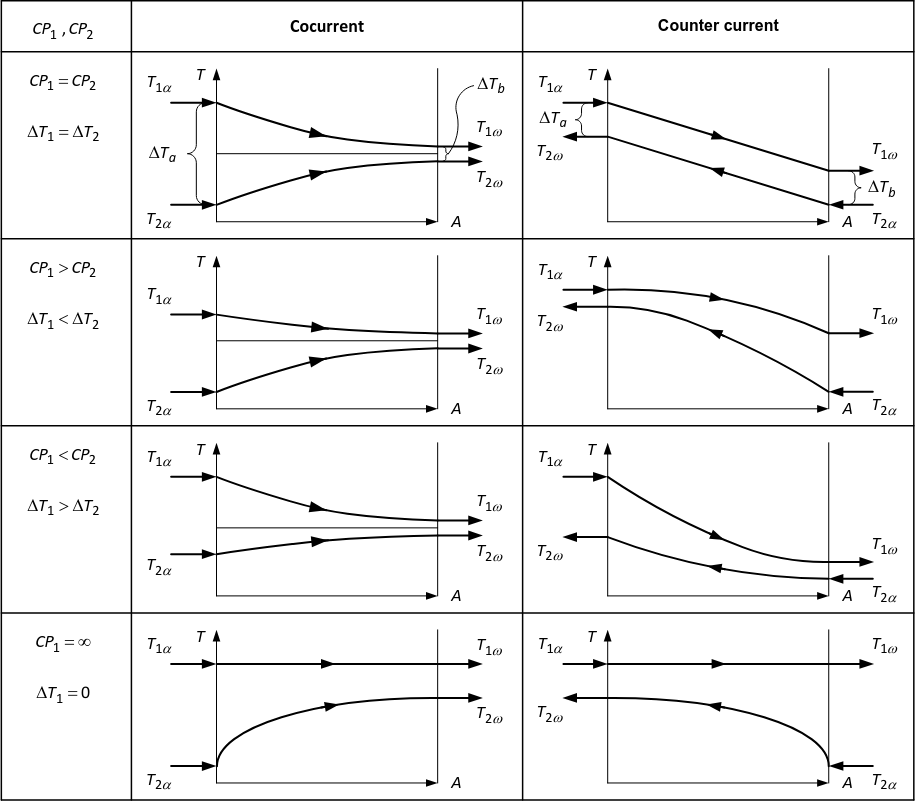
\includegraphics[width=\linewidth]{media/heatexchangers.png}
\end{center}

\subsubsection{Logarithmic mean temperature difference (LMTD)}
\figbox{$\dm \Delta T_m = \dfrac{\Delta T_a - \Delta T_b}{\ln\dfrac{\Delta T_a}{\Delta T_b}}$}
\[\Delta T_a = \left|\vartheta_{1,a} - \vartheta_{2,a}\right|\quad ; \quad \Delta T_b = \left|\vartheta_{1,b} - \vartheta_{2,b}\right|\]

\subsubsection{Corrected mean temperature heat flow}
\begin{center}
  \fbox{$\dot{Q} = kA\Delta T_m \cdot F_T$} , with $0 < F_T < 1$
\end{center}

\begin{center}
  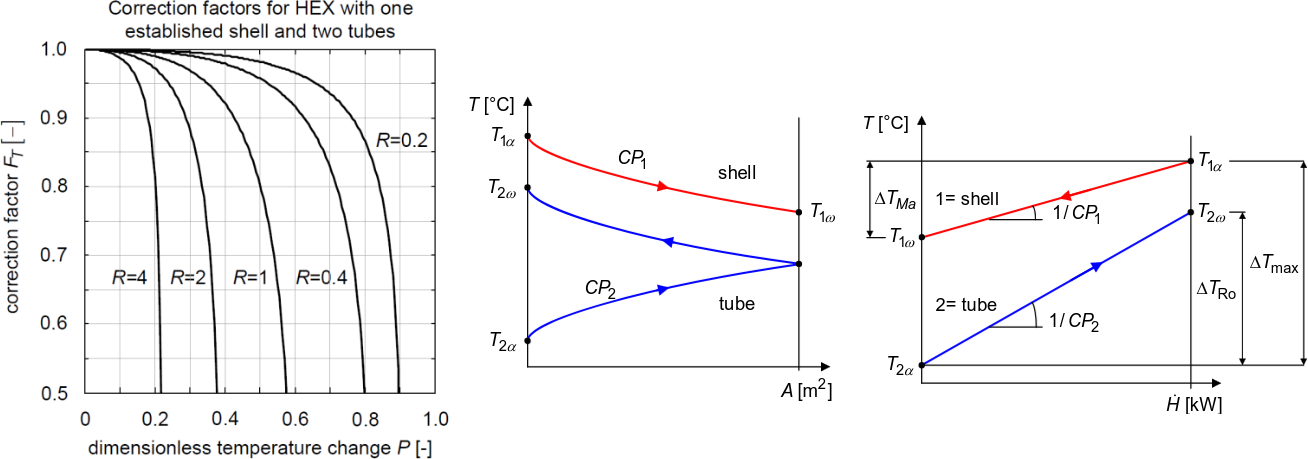
\includegraphics[\lw=.9]{media/HEXcorrection.png}
\end{center}

\subsection{Co-current vs countercurrent flow heat exchanger}
\begin{gather*}
  \dot{Q} = kA_\text{co}\Delta T_{m,\text{co}} = kA_\text{count}\Delta T_{m,\text{count}}\\
  \dfrac{A_\text{co}}{A_\text{count}} = \dfrac{\Delta T_{m,\text{count}}}{\Delta T_{m,\text{co}}}\\[1ex]
  \dfrac{A_\text{co}}{A_\text{count}} = \dfrac{\dot{Q}_\text{co}}{\dot{Q}_\text{count}}\cdot \dfrac{\Delta T_{m,\text{count}}}{\Delta T_{m,\text{co}}},\quad \text{if } \dot{Q}_1 \neq \dot{Q}_2
\end{gather*}

\subsection{Heat capacity rate ratio (Capacity ratio)}
It measures the relative ability of stream 1 vs. stream 2 to carry
heat per kelvin:
\begin{gather*}
  CP_1 \left(\vartheta_{1, \alpha} - \vartheta _{1, \omega}\right) = CP_2 \left(\vartheta_{2\omega} - \vartheta_{2,\alpha}\right)\\[1ex]
  R_1 = \dfrac{CP_1}{CP_2} = \dfrac{\vartheta_{2,\omega} - \vartheta_{2,\alpha}}{\vartheta_{1,\alpha}-\vartheta_{1,\omega}} = \dfrac{\Delta \vartheta_2}{\Delta \vartheta_1}
\end{gather*}

\section{T,H diagram}
\subsection{Cold and Hot streams}
The process is extracted into material streams that must be heated
(heating need) or cooled (cooling need):
\begingroup
\renewcommand{\arraystretch}{1.25}
\footnotesize
\begin{tabularx}{\linewidth}{|>{\raggedright\arraybackslash}X|>{\raggedright\arraybackslash}X|}
  \hline
  \textbf{\textcolor{blue}{Cold streams}}
  & \textbf{\textcolor{red}{Hot streams}} \\
  \hline
  \begin{minipage}[t]{\linewidth}
    Heating needed (heat sink):
    \begin{itemize}[nosep,leftmargin=*]
      \item Warming of milk for pasteurisation
      \item Heating a heat transfer oil
      \item Preparation of hot water
      \item Evaporation of fruit juice
    \end{itemize}
  \end{minipage}
  &
  \begin{minipage}[t]{\linewidth}
    Cooling needed (heat source)
    \begin{itemize}[nosep,leftmargin=*]
      \item Cooling of a salt solution
      \item Cooling a polymer melt
      \item Cooling water from air compressors
      \item Chiller refrigerant
      \item Flue gas
    \end{itemize}
  \end{minipage} \\
  \hline
\end{tabularx}
\endgroup

\begin{center}
  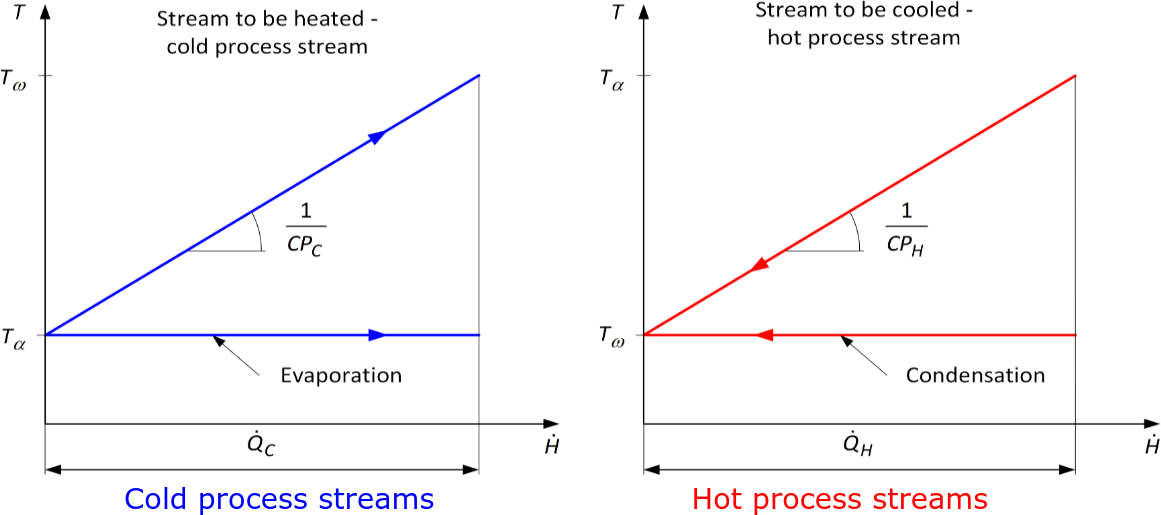
\includegraphics[\lw]{media/C,H streams.png}
\end{center}

\subsubsection{Slope of the streams}
\begin{gather*}\dm
  \frac{\Delta T}{\Delta \dot{H}} \Longleftrightarrow \frac{\Delta T_1}{CP_1 \cdot \Delta T_1} = \frac{1}{CP_1} \Longleftrightarrow \frac{\Delta T_2}{CP_2 \cdot \Delta T_2} = \frac{1}{CP_2}
\end{gather*}

\subsection{Composite curve}
\figbox{$\dm \frac{1}{CP_n} = \frac{\Delta T_n}{\Delta \dot{H}_n} = \frac{\Delta T_n}{\sum_i CP_i \Delta T_n} = \frac{1}{\sum_i CP_i}$}

\begin{center}
  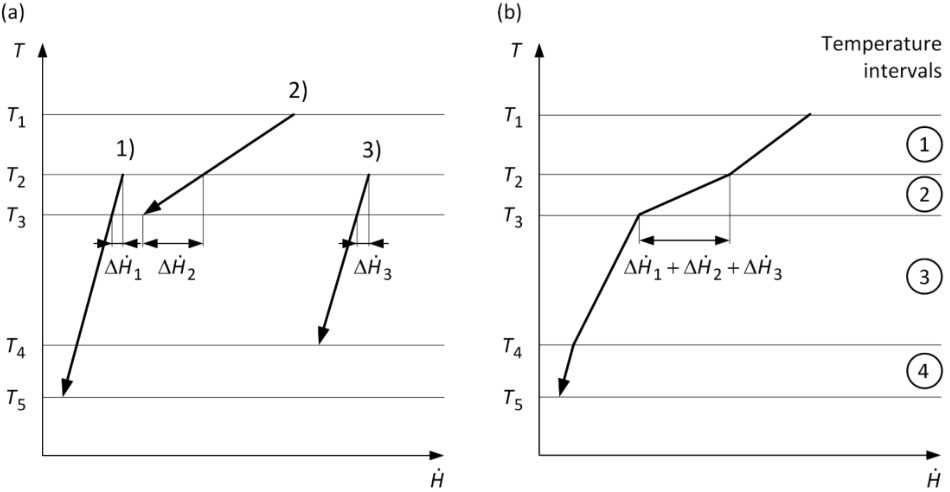
\includegraphics[\lw=.8]{media/composite-curve.png}
\end{center}

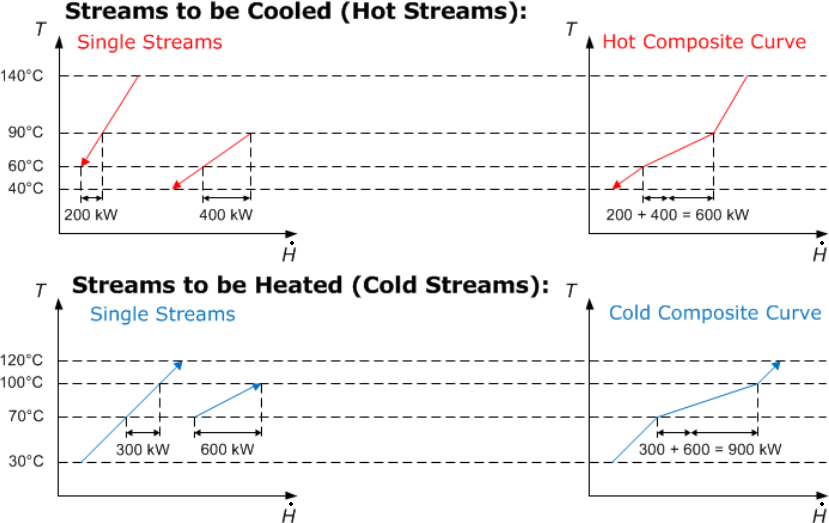
\includegraphics[\lw]{media/composite-curve2.png}

\part{Energy and Cost Targets}
\noindent\resizebox{\linewidth}{!}{%
\begin{tabular}{|l|c|c|c|c|c|}
  \hline $\Delta T_\text{min}$ & \makecell{HR\\Potential} & \makecell{Required\\Utilities} & \makecell{HEX\\Area} & \makecell{Investments\\Costs} & \makecell{Energy\\Costs} \\
  \hline decreases & increases & decreases & increases & increases & decreases \\
  \hline increases & decreases & increases & decreases & decreases & increases \\
  \hline 
\end{tabular}%
}

\section{Cost targets}
\subsection{Calculation of Annual Total Costs (Annualized Total Costs)}
\figbox{$C_\text{tot} = AC_\text{inv} + C_\text{Op}$}

\subsection{Annuity factor}
\[A=\dfrac{Z(1+Z)^n}{(1+Z)^n - 1}\]

$Z$ = interest rate\\
$n$ = Depreciation/Amortisation period 

\subsection{Investment costs}
\[C_\text{Inv} = C_\text{HEN} + C_\text{ECU} + C_\text{Ind}\]

HEN = Heat exchanger network cost\\
ECUs = Energy conversion units\\
Ind = Independent (eg. control integration)

\subsubsection{Capital costs for heat exchanger network (HEN)}
\[C_\text{HEN} = \sum C_\text{HEX} = \sum\left(a + C_b\left(\dfrac{Q}{Q_b}\right)^m\right)\]

\begin{tabularx}{\linewidth}{@{}lX@{}}
  $C_\text{HEX}$ & Capital cost of heat exchanger (HEX) \\
  $a$ & Base cost \\
  $C_b$ & Cost of reference heat exchanger \\
  $Q_b$ & Heat transfer area of reference heat exchanger \\
  $m$ & Degression exponent \\
  $Q$ & Area of HEX to be costed
\end{tabularx}

$Q$ refers to quantity (in this case, Area for the HEX costs)

\subsection{Annual operating costs}
\[C_\text{Op} = C_\text{En} + C_\text{M} + C_\text{Per}\]

\subsubsection{Maintenance costs}
\[C_\text{M} = C_\text{Inv}f_\text{M}\]

\subsubsection{Personnel costs}
\[C_\text{Per} = C_\text{Inv}f_\text{Per}\]

\subsection{Annual energy costs}
Annual energy costs are the sum of the annual hot and cold utility costs and the energy costs of the ECUs.
\[C_\text{En} = C_\text{HU} + C_\text{CU} + C_{\text{En,ECU}}\]

\subsubsection{Hot utility costs}
\[C_\text{HU} = \dot{Q}_\text{HU}\tau c_\text{HU}\]

\subsubsection{Cold utility costs}
\[C_\text{CU} = \dot{Q}_\text{CU}\tau c_\text{CU}\]

\begin{tabularx}{\linewidth}{@{}lX@{}}
  $\dot{Q}_{\text{HU/CU}}$ & Hot/cold utility requirements (heat flow rate) \\
  $C_{\text{HU/CU}}$ & Annual energy cost of hot/cold utility \\
  $\tau$ & Annual operating hours \\
  $c_{\text{HU/CU}}$ & Specific energy cost of hot/cold utility
\end{tabularx}

\subsubsection{Energy costs of energy conversion units (ECUs)}
\[C_{\text{En,ECU}} = \sum E_\text{ECU}c_\text{En}\]

\begin{tabularx}{\linewidth}{@{}lX@{}}
  $C_{\text{En,ECU}}$ & Annual energy cost of ECUs \\
  $E_\text{ECU}$ & Annual energy requirement of an ECU \\
  $c_\text{En}$ & Specific cost of the energy supplied to an ECU
\end{tabularx}

\subsection{Heat exchanger network cost target}
Assuming an equal distribution of the total heat transfer area among the required heat exchangers:
\[
  C_{\text{HEN,Target}} = N_{\text{Units,Target}}
  \left(a + C_b\left(
    \frac{A_{\text{HEN,Target}}}{N_{\text{Units,Target}}Q_b}
  \right)^m\right)
\]

\subsubsection{Single-stream heat transfer area target}
\[
  A_{\text{HEN,Target}} = \frac{\dot{Q}}{\Delta T_m}
  \left(\frac{1}{\alpha_h} + \frac{1}{\alpha_c}\right)
\]

\subsubsection{Heat transfer area target (Uniform Bath Formula)}
\[
  A_{\text{HEN,Target}} = \sum_{k=1}^{K}\frac{1}{\Delta T_{m,k}}
  \left[
    \sum_{i=1}^{I}\frac{\dot{Q}_{i,k}}{\alpha_i}
    + \sum_{j=1}^{J}\frac{\dot{Q}_{j,k}}{\alpha_j}
  \right]
\]

\begin{tabularx}{\linewidth}{@{}lX@{}}
  $k,K$ & Enthalpy interval index $k$ through $K$ \\
  $i,j$ & Hot and cold stream indices within interval $k$ \\
  $I,J$ & Number of hot and cold streams within interval $k$ \\
  $\alpha_i,\alpha_j$ & Heat transfer coefficients of hot and cold streams \\
  $\dot{Q}_{i,k},\dot{Q}_{j,k}$ & Heat flow rates of the streams within interval $k$ \\
  $\Delta T_{m,k}$ & Mean temperature difference within interval $k$ \\
  $A_{\text{HEN,Target}}$ & Target total heat transfer area of the HEN
\end{tabularx}

\subsubsection{Number of heat exchangers}
\[N_{\text{Units,Target}} = [S_\text{above}-1] + [S_\text{below}-1]\]

\begin{tabularx}{\linewidth}{@{}lX@{}}
  $N_{\text{Units,Target}}$ & Target number of heat exchangers \\
  $S_\text{above}$ & \footnotesize Number of streams including utilities above the pinch \\
  $S_\text{below}$ & \footnotesize Number of streams including utilities below the pinch
\end{tabularx}

\section{Energy targets}
\subsection{Three main pinch rules}
\figbox{\begin{enumerate}
  \item No heat transfer through the pinch
  \item No external heating below the pinch
  \item No external cooling above the pinch
\end{enumerate}}

\subsection{Characteristics of the pinch point}
The pinch divides the total system into two subsystems with:
\vspace*{-.2cm}
\begin{itemize}
  \item Heat deficit above the pinch
  \item Heat excess below the pinch.
\end{itemize}

\begin{center}
  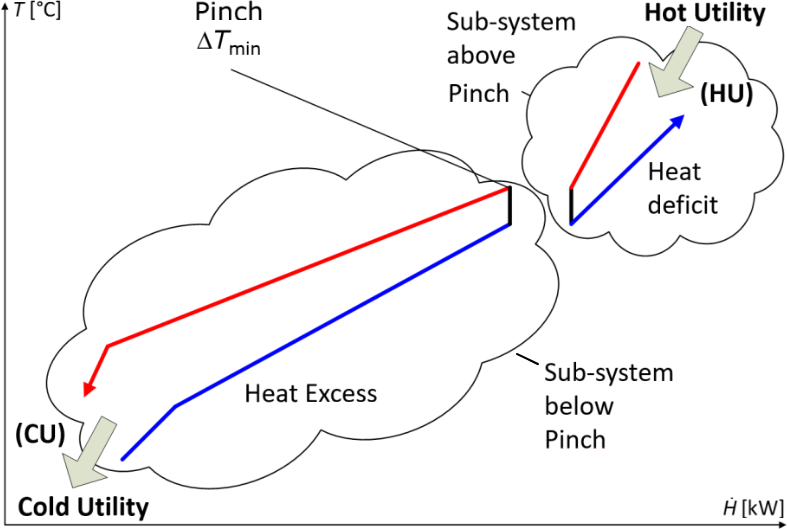
\includegraphics[\lw=.8]{media/above-below-pinch.png}
\end{center}

\newcolumn
\part{Heat Exchanger Network (HEN)}
MER = Maximum Energy Recovery (for HR)\\
MER = Minimum Energy Requirement (for CU/HU)\\[1ex]
Inwards = Stream that is approaching the PT\\
Outwards = Stream temperature that is leaving the PT

\section{Rules for the design of HENs}
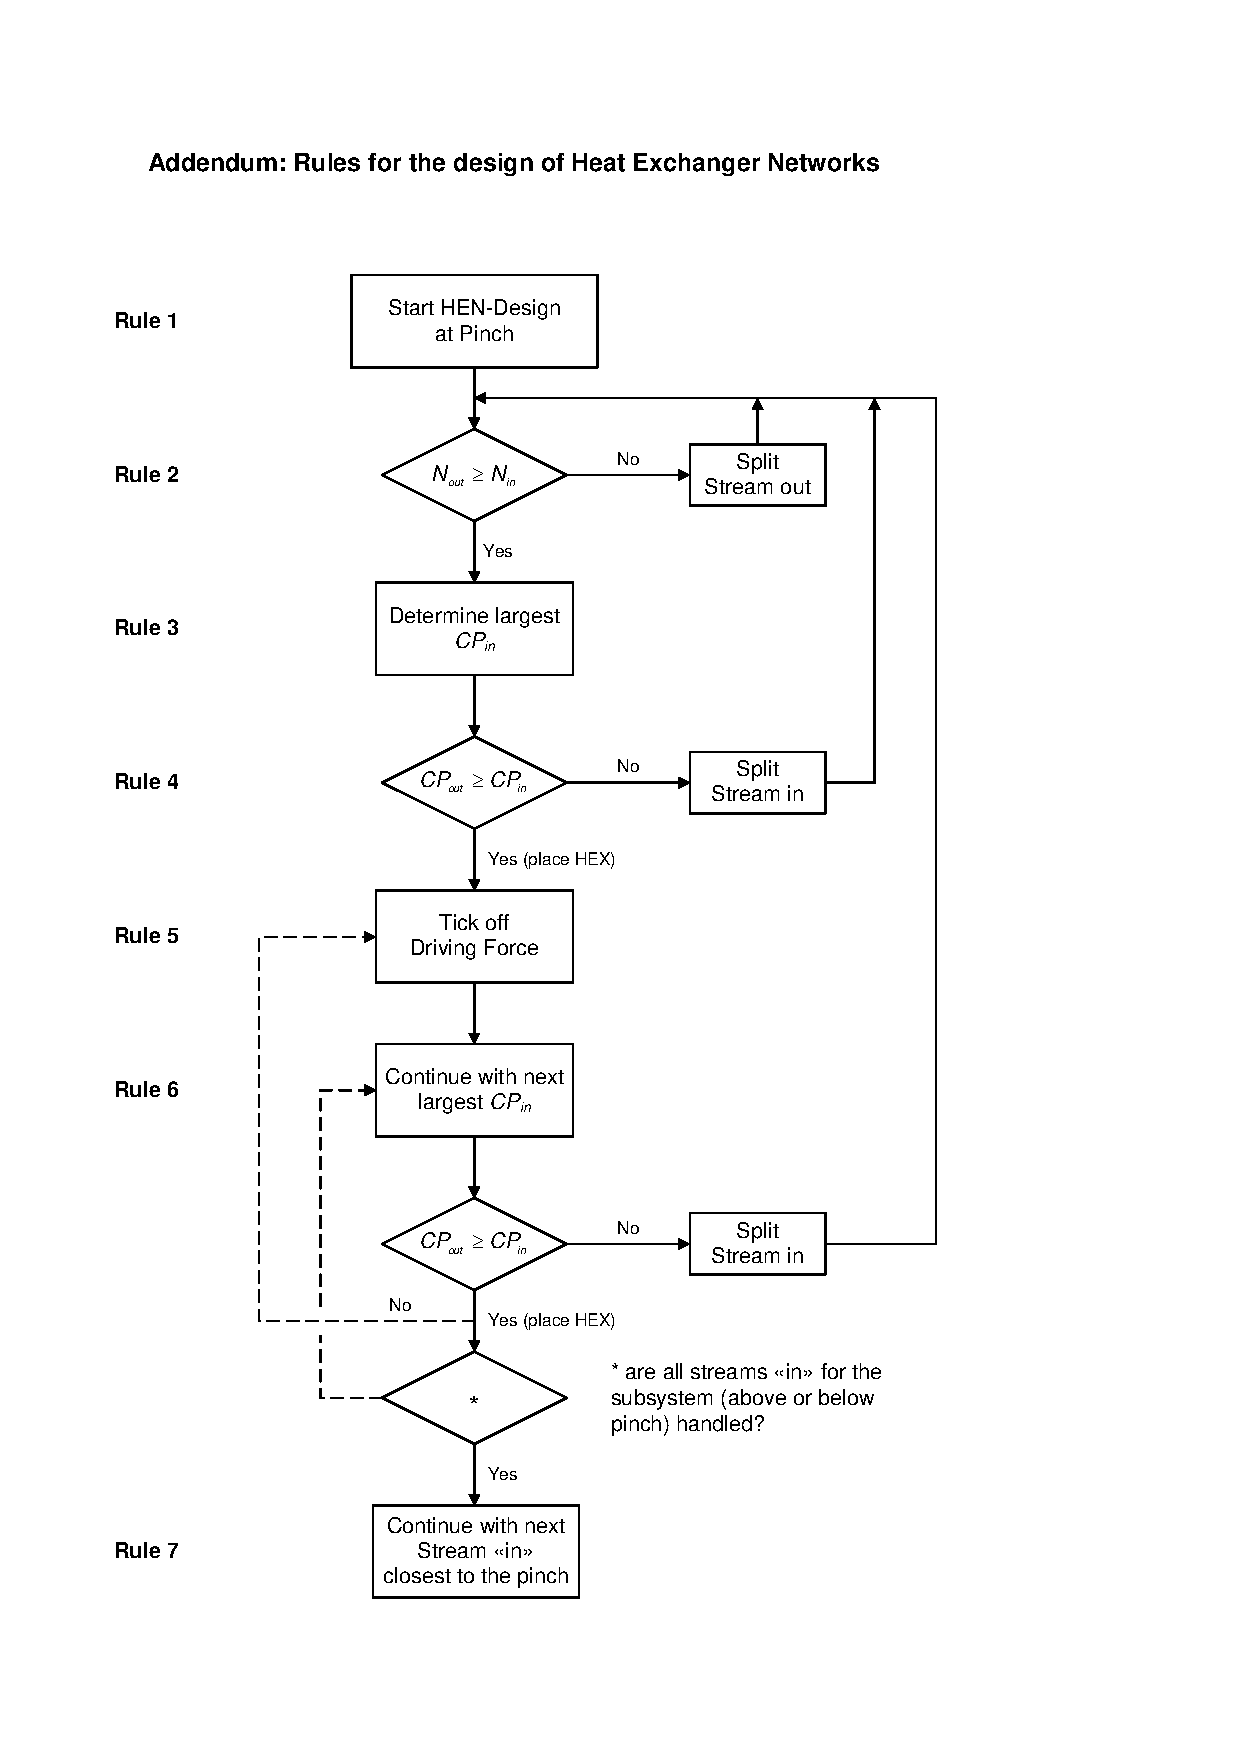
\includegraphics[\lw]{media/Addendum HEN Design Rules.pdf}

\newcolumn
These design rules help to achieve the targets.
\begin{enumerate}
  \item Start from the pinch and progress outwards
  \item Number rule: $N_\text{out} \geq N_\text{in}$ : every stream which heads in the direction of the pinch has a match partner in a HEX
  \item Begin with the largest $CP_\text{in}$ : stream which heads in the direction of the pinch with the largest $CP_\text{in}$
  \item $CP$ rule: $CP_\text{out} \geq CP_\text{in}$ : no HEX less than $\Delta T_\text{min}$
  \item HEX Optimization:
  \begin{enumerate}[label=\alph*)]
    \item \textcolor{red}{\textbf{``Tick Off Rule''}}: minimize the number of HEX and/or
    \item \textcolor{red}{\textbf{``Driving Force Plot''}}: minimize the area of the HEN
  \end{enumerate}
  \item Continue with the largest $CP_\text{in}$ at the Pinch
  \item If all HEXs at the Pinch are set, then proceed with the stream closest to the Pinch that leads to the Pinch
\end{enumerate}

\part{Process requirements}
{\color{red}TODO}

\part{Optimizing energy supply systems (ESS)}
\section{Optimizing utilities ESS}
\subsection{Grand Composite Curve (GCC)}
GCC is formed from the Composite Curves (CC) and applies only for
a certain $\Delta T_\text{min}$.

To construct the GCC, the CCs are each shifted vertically by $\dm \pm\frac{\Delta T_\text{min}}{2}$
until they touch at the pinch point.
\begin{center}
  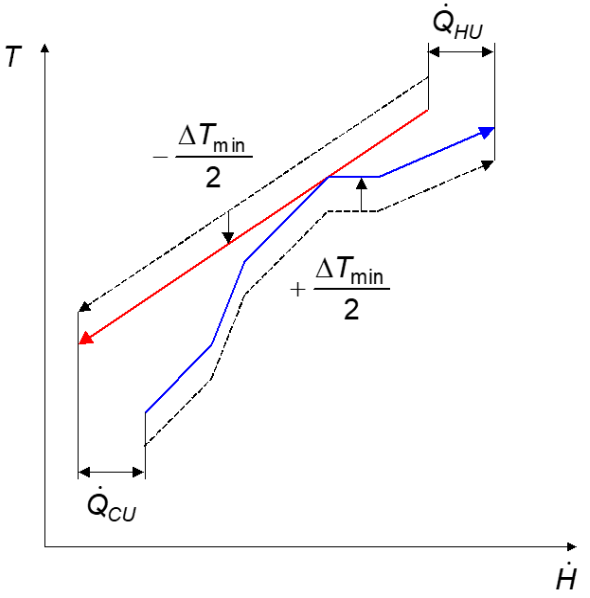
\includegraphics[\lw=.7]{media/GCC.png}
\end{center}
The horizontal distance correspond to the required hot and cold utilities.

The horizontal distance between the shifted CCs are transferred into another $T,\dot H$-diagram
\begin{center}
  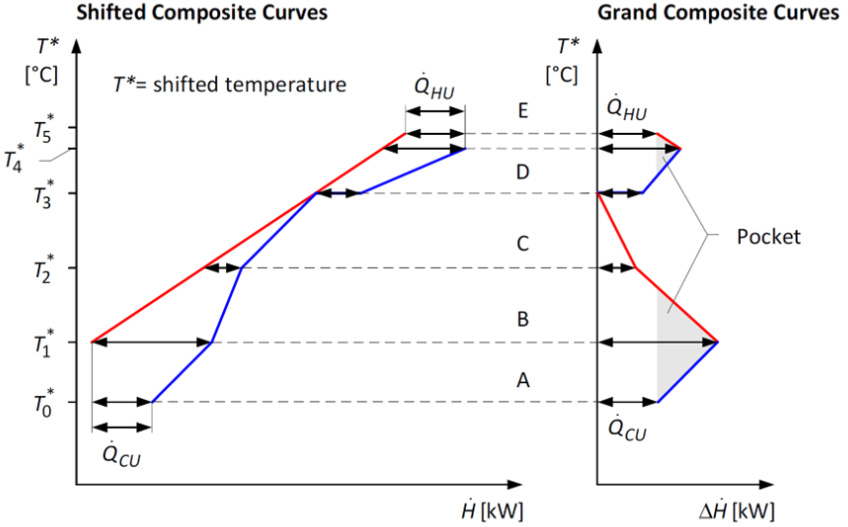
\includegraphics[\lw]{media/shifted-GCC.png}
\end{center}

\subsubsection{Pockets in the GCC}
Pockets show internal heat recovery. Heat released at higher temperatures
supplies process heat demand at lower temperatures, without external utilities.

\subsubsection{Optimization of the utility system temperature levels}
Calculation of the real temperature of the hot utility from the optimized
shifted temperature, according to the GCC:
\[T_{HU} = T^*_{HU} + \frac{\Delta T_\text{min}}{2}\quad ; \quad T_{CU} = T^*_{CU} - \frac{\Delta T_\text{min}}{2}\]

\begin{center}
  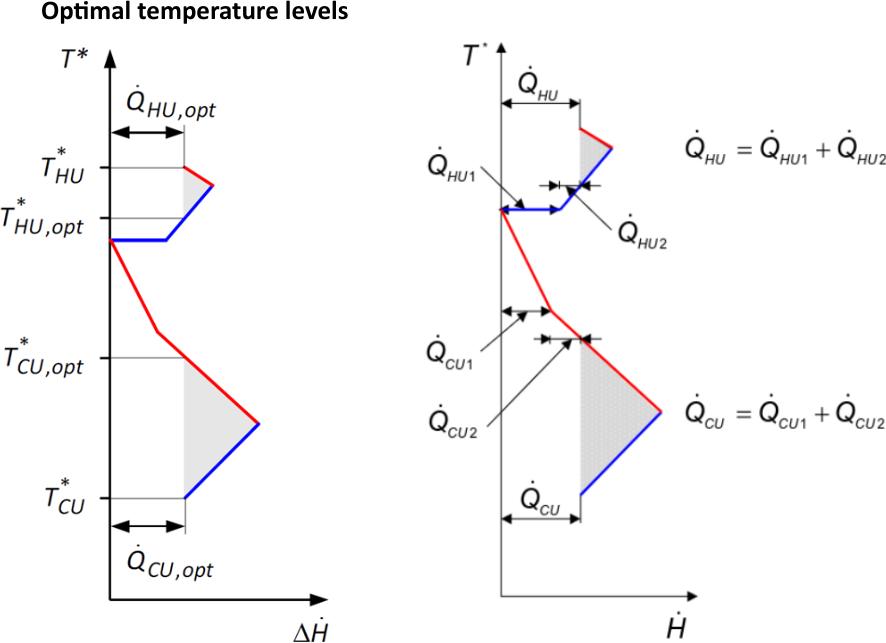
\includegraphics[\lw]{media/optimal-GCC.png}
\end{center}

\section{Utility optimization and consequences for the HEN design}
HEN has to be constructed on the CCs including the utilities\\
$\to$ Balanced Composite Curve (BCC)

\subsection{Balanced Composite Curves (BCCs) and BGCCs}
\begin{center}
  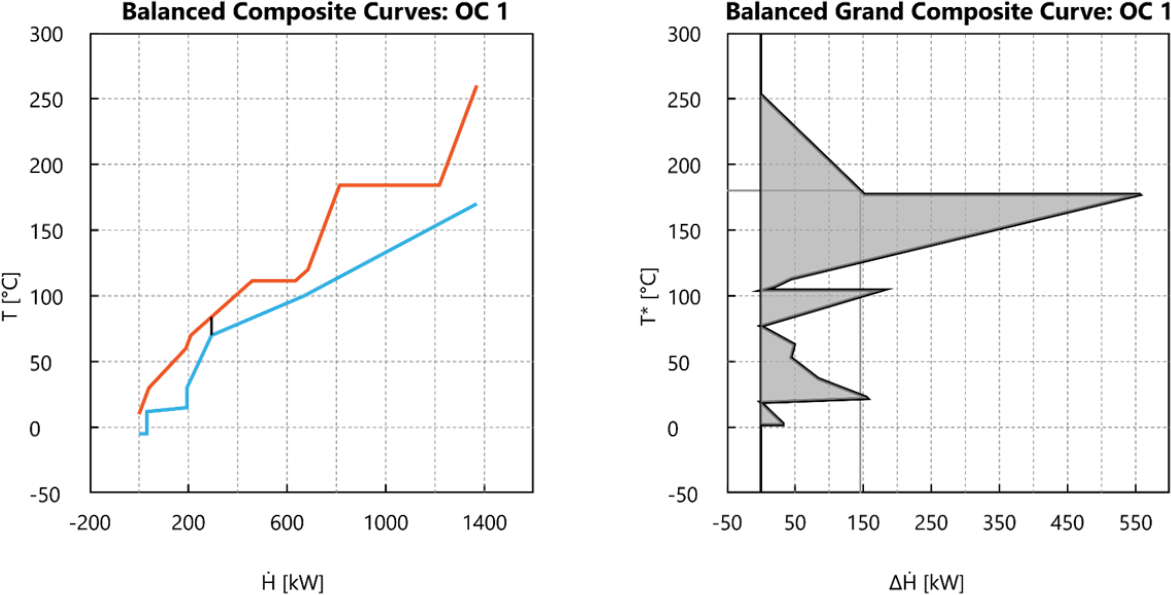
\includegraphics[\lw]{media/BCC.png}
\end{center}

\figbox{\begin{enumerate}
  \item The pinch rules must be applied at the Utility-Pinch
  \item Between two pinches is a clash of the pinch rules
  \item Always start at the most constaint pinch
\end{enumerate}}

\newpage
\part{Integrating ECUs}
ECU = Energy Conversion Unit

\begin{center}
  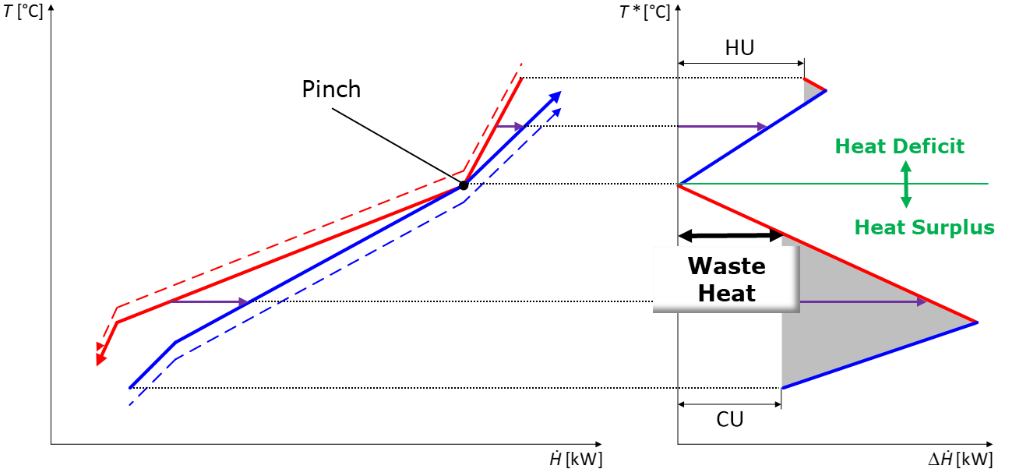
\includegraphics[\lw]{media/GCC-complete.png}
\end{center}

\section{Combined Heat and Power (CHP) systems}
\begin{itemize}
  \item Thermal engines generate electrical energy and heat
  \item $\eta_\text{el}$ 30-40\%, $\eta_\text{tot}$ 80-90\%
  \item Typical CHP: gas turbine, steam turbine, combustion engine
\end{itemize}

\subsection{Integrating CHP}
\begin{center}
  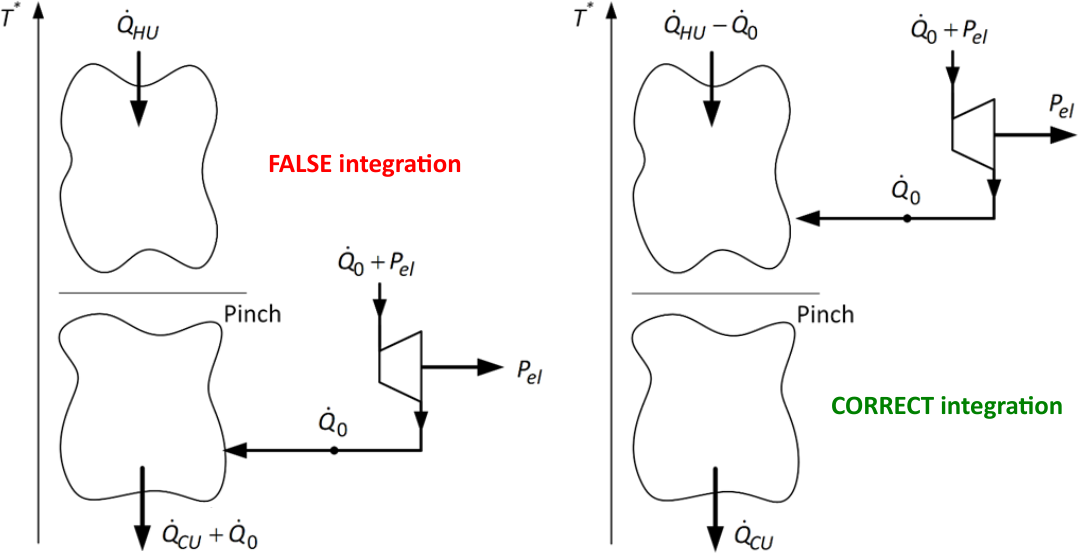
\includegraphics[\lw]{media/CHP-integration.png}
\end{center}

\subsubsection{False integration -- Below the Pinch}
The heat surplus is increased by the amount of heat generated
by the CHP. This results in a higher cooling requirement.

\subsubsection{Correct integration -- Above the Pinch}
The heat deficit is decreased by the amount of heat generated
by the CHP. This results in a decrease of the heating requirement.

\subsection{Method to integrate a steam turbine}
\begin{center}
  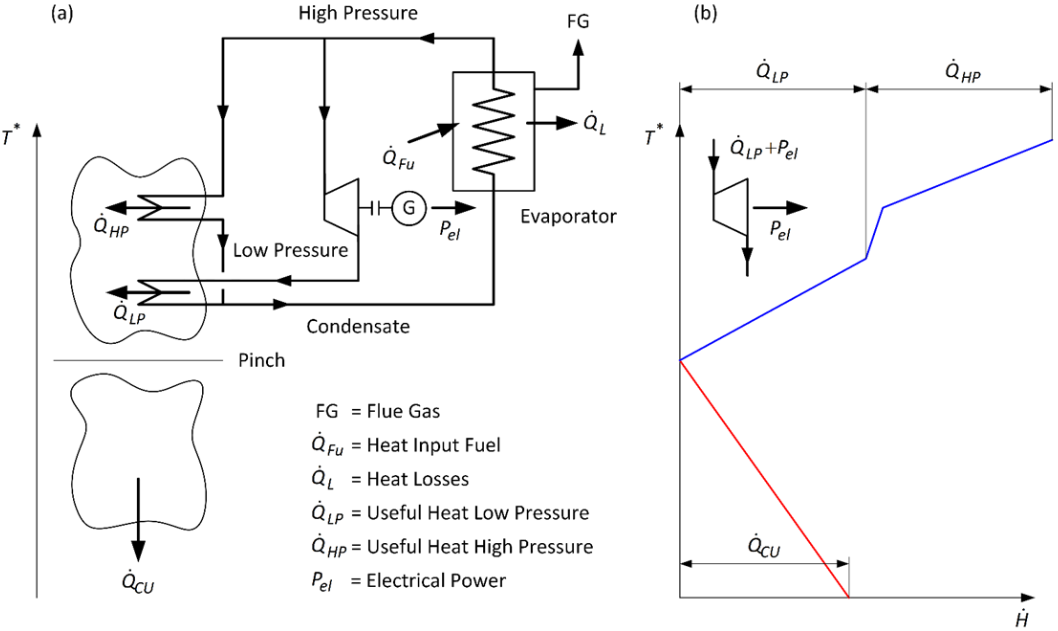
\includegraphics[\lw]{media/CHP-steam.png}
\end{center}

\subsection{Method to integrate a gas turbine}
\begin{center}
  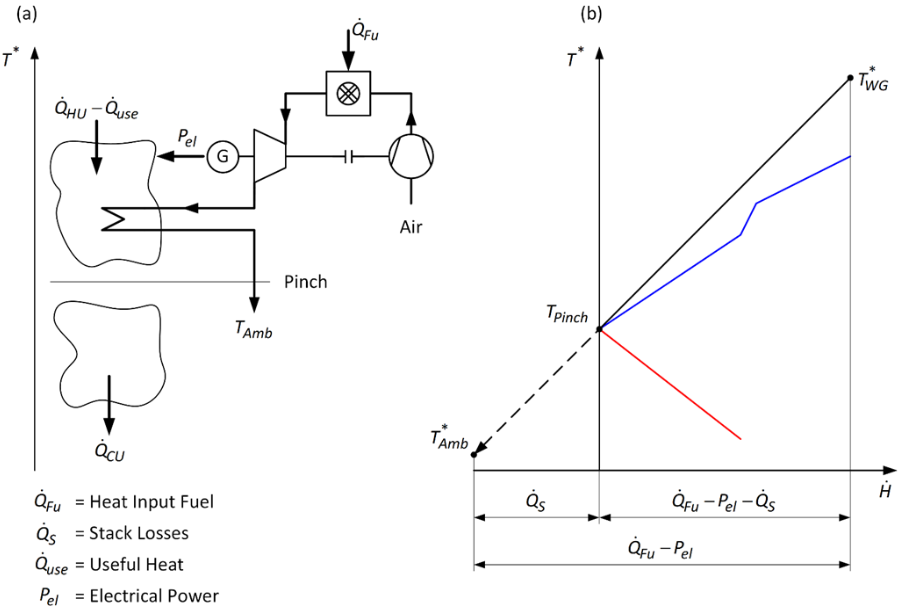
\includegraphics[\lw]{media/CHP-gas.png}
\end{center}

\subsection{Organic Rankine Cycle (ORC) Systems}
Basics:\\
1 \to 2: adiabatic (polytropic) compression\\
2 \to 3: isobaric heat input (high temperature level)\\
3 \to 4: adiabatic expansion\\
4 \to 1: isobaric heat output (low temperature level)
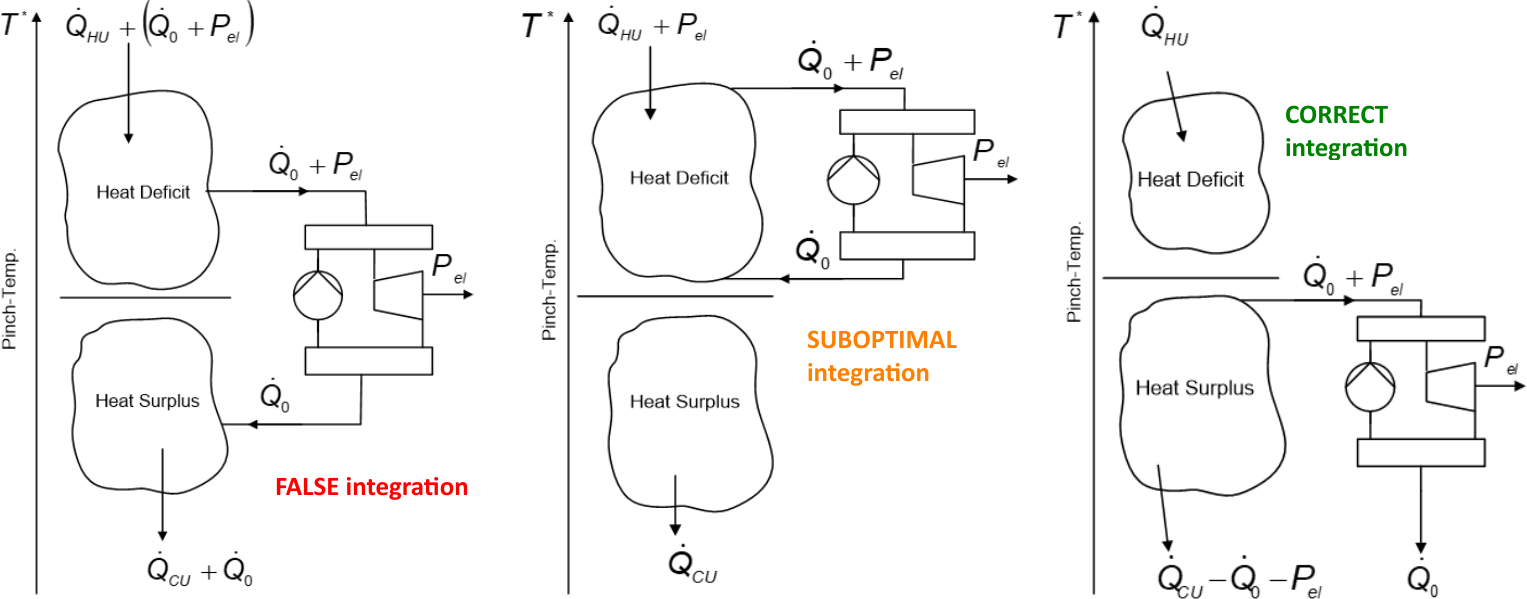
\includegraphics[\lw]{media/ORC-integration.png}

\subsubsection{False integration -- Over the Pinch}
The heat deficit is increased by the amount of electrical power
generated and condenser heat. The heat surplus is increased
by the amount of condenser heat. Both a higher heating and
cooling requirement results.

\subsubsection{Suboptimal integration -- Above the Pinch}
The heat deficit is increased by the amount of electrical power
generated leading to a higher heating requirement

\subsubsection{Correct integration -- Below the Pinch}
The ORC reduces the cooling demand of the process and the
associated operating costs.

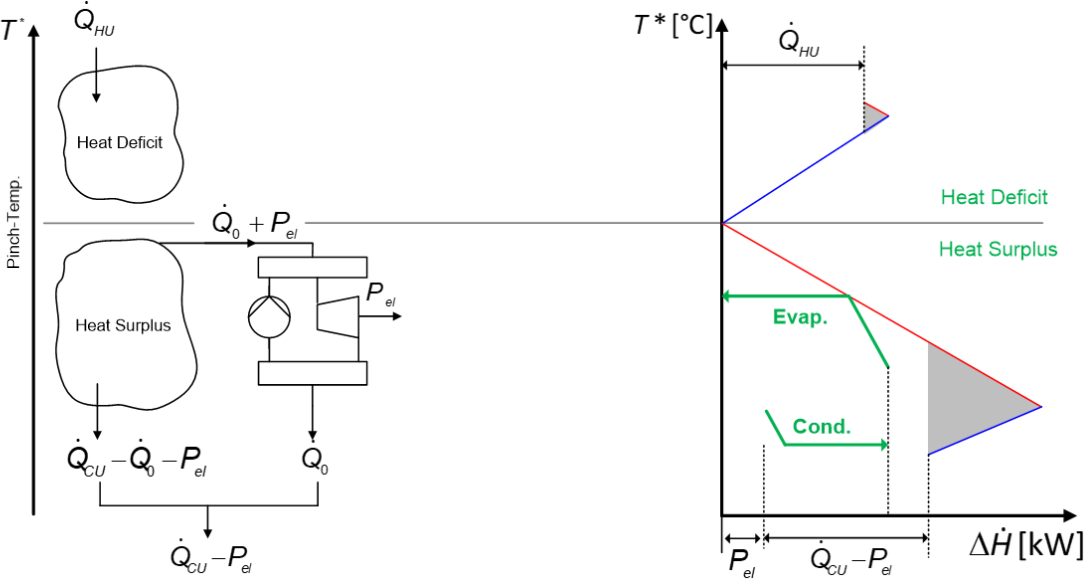
\includegraphics[\lw]{media/ORC.png}

\subsection{Integrating Heat Pumps (HP)}
Basics:\\
1 \to 2: adiabatic (polytropic) compression\\
2 \to 3: isobaric heat output (high temperature level)\\
3 \to 4: adiabatic expansion\\
4 \to 1: isobaric heat input (low temperature level)

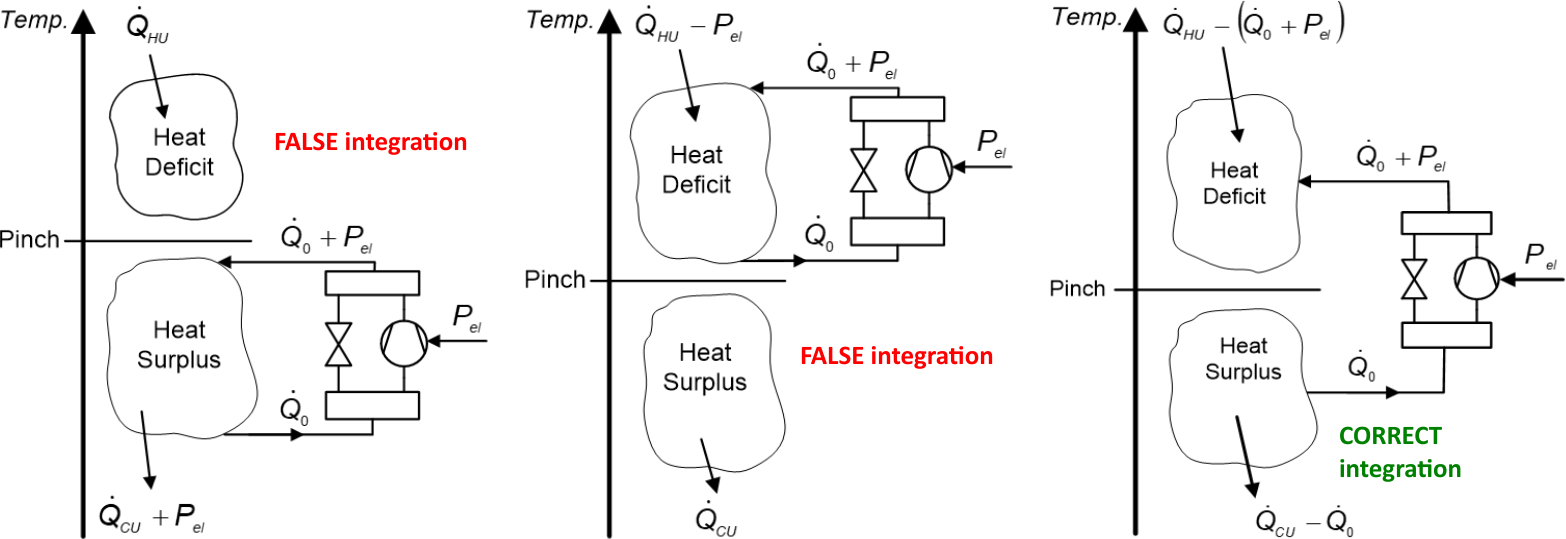
\includegraphics[\lw]{media/HP-integration.png}

\subsubsection{False integration -- Below the Pinch}
The heat surplus is increased by the amount of compressor
electrical power leading to a higher cooling requirement.

\subsubsection{False integration -- Above the Pinch}
The heat deficit is reduced by the amount of compressor
electrical power. From an energetic perspective this type of
integration is equivalent to electrical heating.

\subsubsection{Correct integration -- Over the Pinch}
The heat pump reduces both the cooling and the heating
demands of the process and the associated operating costs.

\subsubsection{Correct integration and basic design using the GCC}
A heat pump may only absorb heat below the pinch (excess heat) and
give off heat above the pinch (heat deficit) to the process.

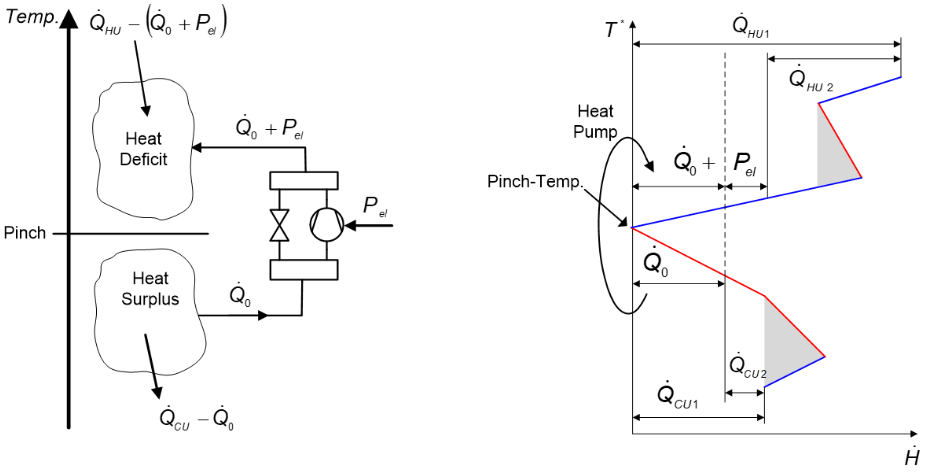
\includegraphics[\lw]{media/HP.png}

\subsubsection{HP integration across the Process Pinch or Utility Pinch}
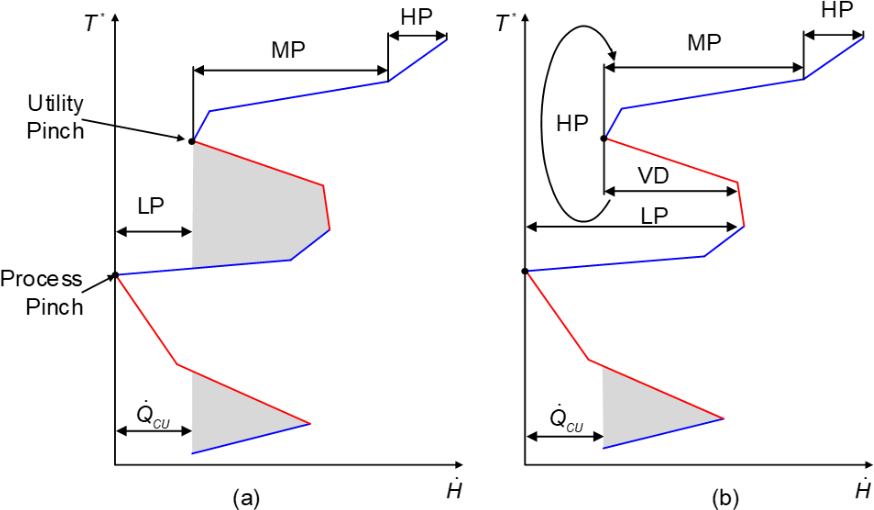
\includegraphics[\lw]{media/HP-integration2.png}

\subsection{Principle of Mechanical Vapor Recompression (MVR)}
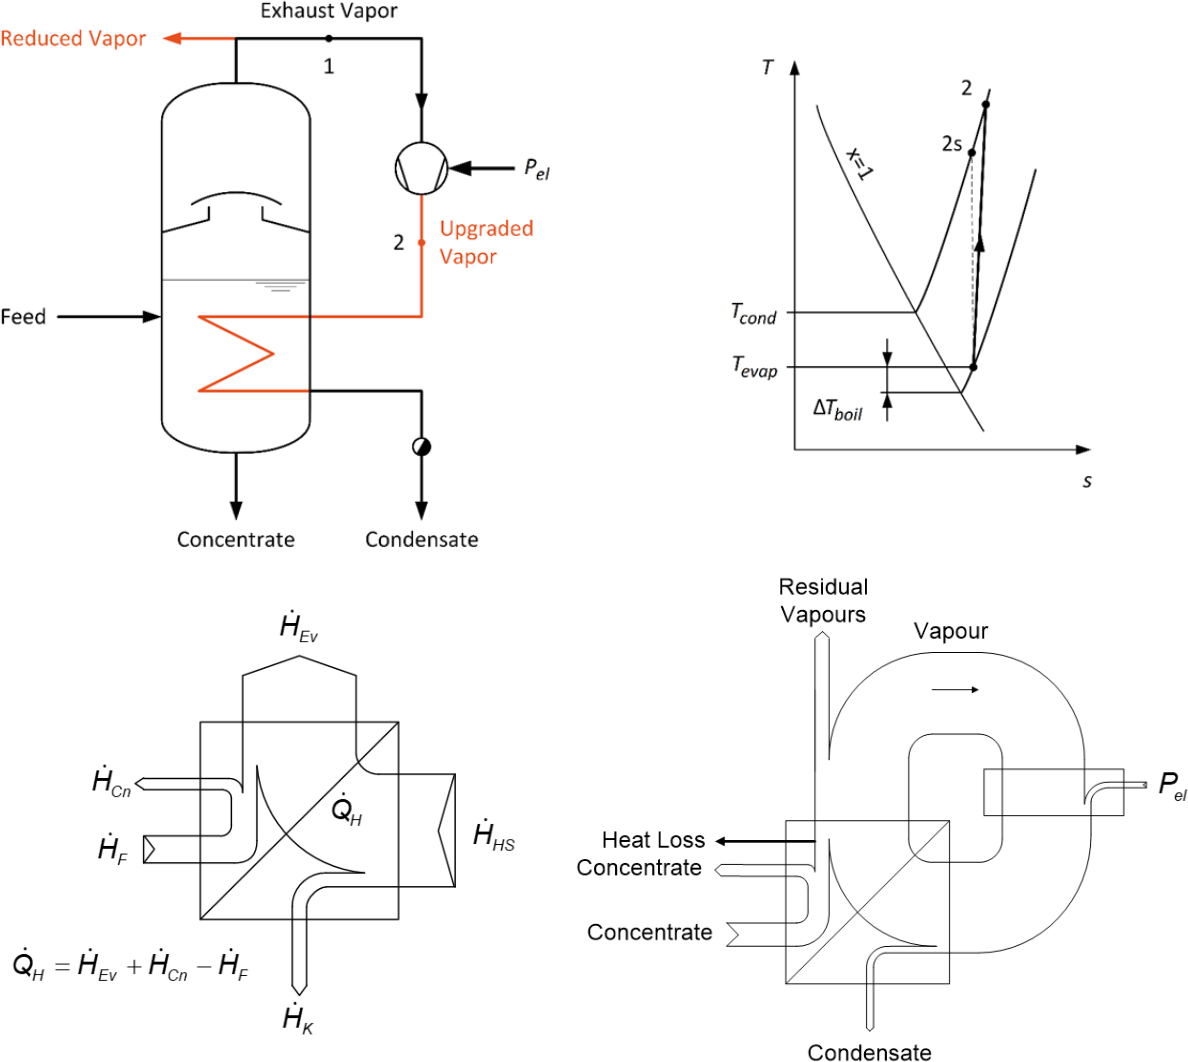
\includegraphics[\lw]{media/MVR.png}

The drive energy of the compressor is usually less than 10\% of the heat
when supplied by direct heating.

\newcolumn
\subsection{Principle of Thermal Vapor Recompression (TVR)}
A typical application of an TVR is for the compression of exhaust steam to a higher pressure
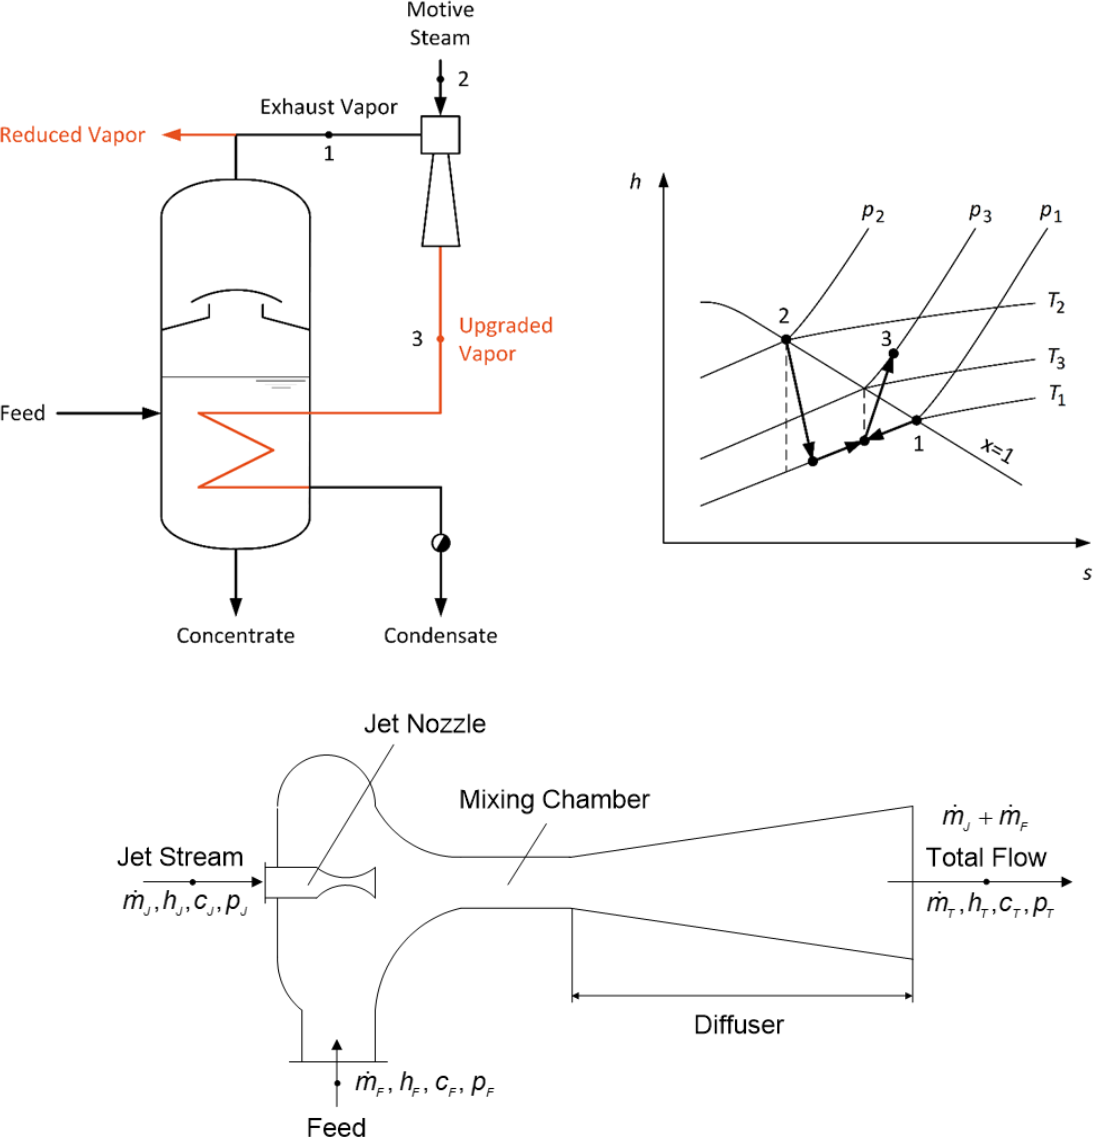
\includegraphics[\lw]{media/TVR.png}

The resulting enthalpy of the resulting mixture of the two steam flows is typically between 3 to 6 times
higher the enthalpy of the exhaust steam! This fact makes a TVR suitable for different energetic situations
than an MVR.

\subsection{Integration of MVR/TVR}
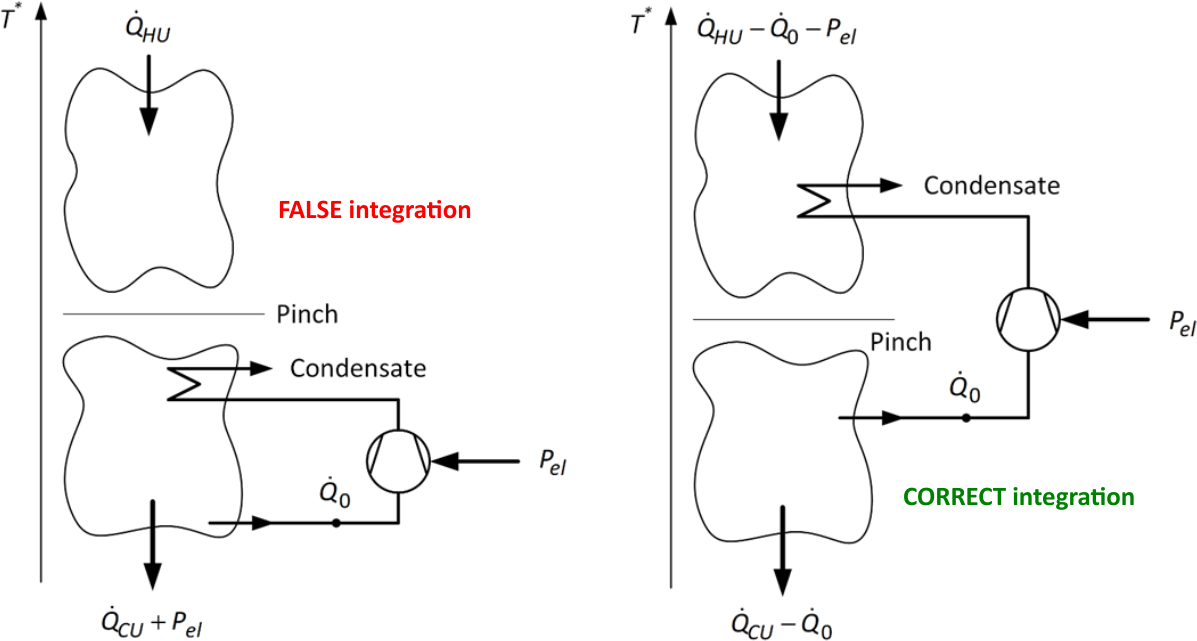
\includegraphics[\lw]{media/VR-integration.png}

\subsubsection{False integration -- Below the Pinch}
The heat surplus is increased by the amount of compressor
electrical power leading to a higher cooling requirement.

\subsubsection{Correct integration -- Over the Pinch}
The MVR/TVR reduces both the cooling and the heating
demands of the process and the associated operating costs.

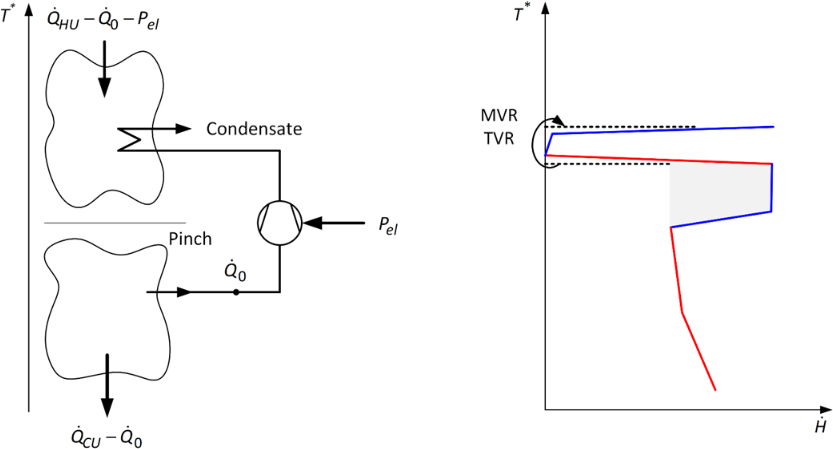
\includegraphics[\lw]{media/VR.png}

A vapor recompression may only absorb heat below the pinch
(excess heat) and give off heat above the pinch (heat deficit).









































\end{multicols*}
\end{document}
